\clearpage
\section{Physical channel3 after confirmed USB move}
The first requested channel3 probe found no response; a control probe confirmed
DAC0/1 still reached4. The owner then confirmed moving both USB cables to3.
Fresh active/inhibited probes verify the J8 ADC route and normal selector map[0,1].
MCU1803, FPGA ff2f746c and power guards passed. No programming, clock changes,
Kasli output release, or repeated timing/SMU tests. Earlier qualified results are unchanged.
\subsection{ADC and adjacent bits: PASS}
Both257-point sweeps span plus/minus1.2V differential at common mode1V,
output legs0.4--1.6V. All bits and44adjacent-pair states exercised.
The frozen source/method contract matches the qualified preceding channels.
\begin{center}\begin{tabular}{lrrr}\toprule
ADC & Gain(code/V) & Zero mean(code) & Template-removed RMS(code)\\\midrule
A & -1781.83 & 2162.019 & 0.535 \\
B & -1780.01 & 2149.342 & 0.509 \\
\bottomrule\end{tabular}\end{center}
\begin{center}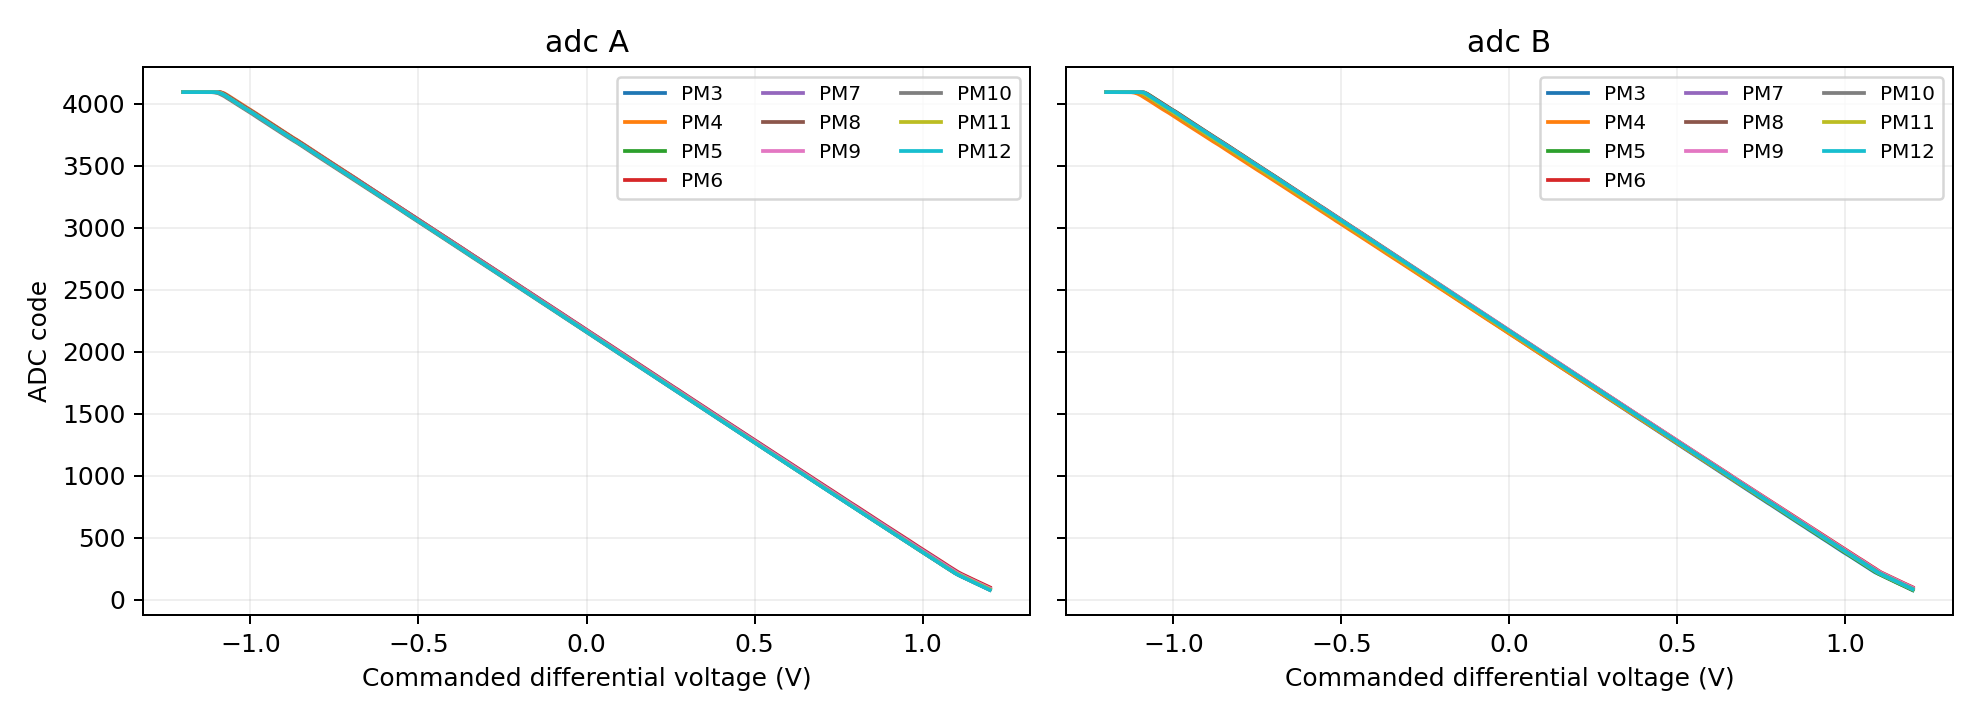
\includegraphics[width=\linewidth]{ch03-adc-common.png}\end{center}
Older10--12 use c7c42d28; newer analog uses ff2f746c. Individual receipts retain
epochs and source versions; commanded voltage is whole-chain response, not ADC-only calibration.
\subsection{Integrator: INCOMPLETE}
The13-point coarse and26-point fine acquisitions completed. BankB retained only one unambiguous fine point; no signed fine crossing could be established, and independent returns did not run. No full integrator PASS or hardware defect is inferred; thresholds unchanged. Independent raw-buffer revalidation retained 26 of26fine points on A and1of26 on B. The separation threshold remains30codes.
\begin{center}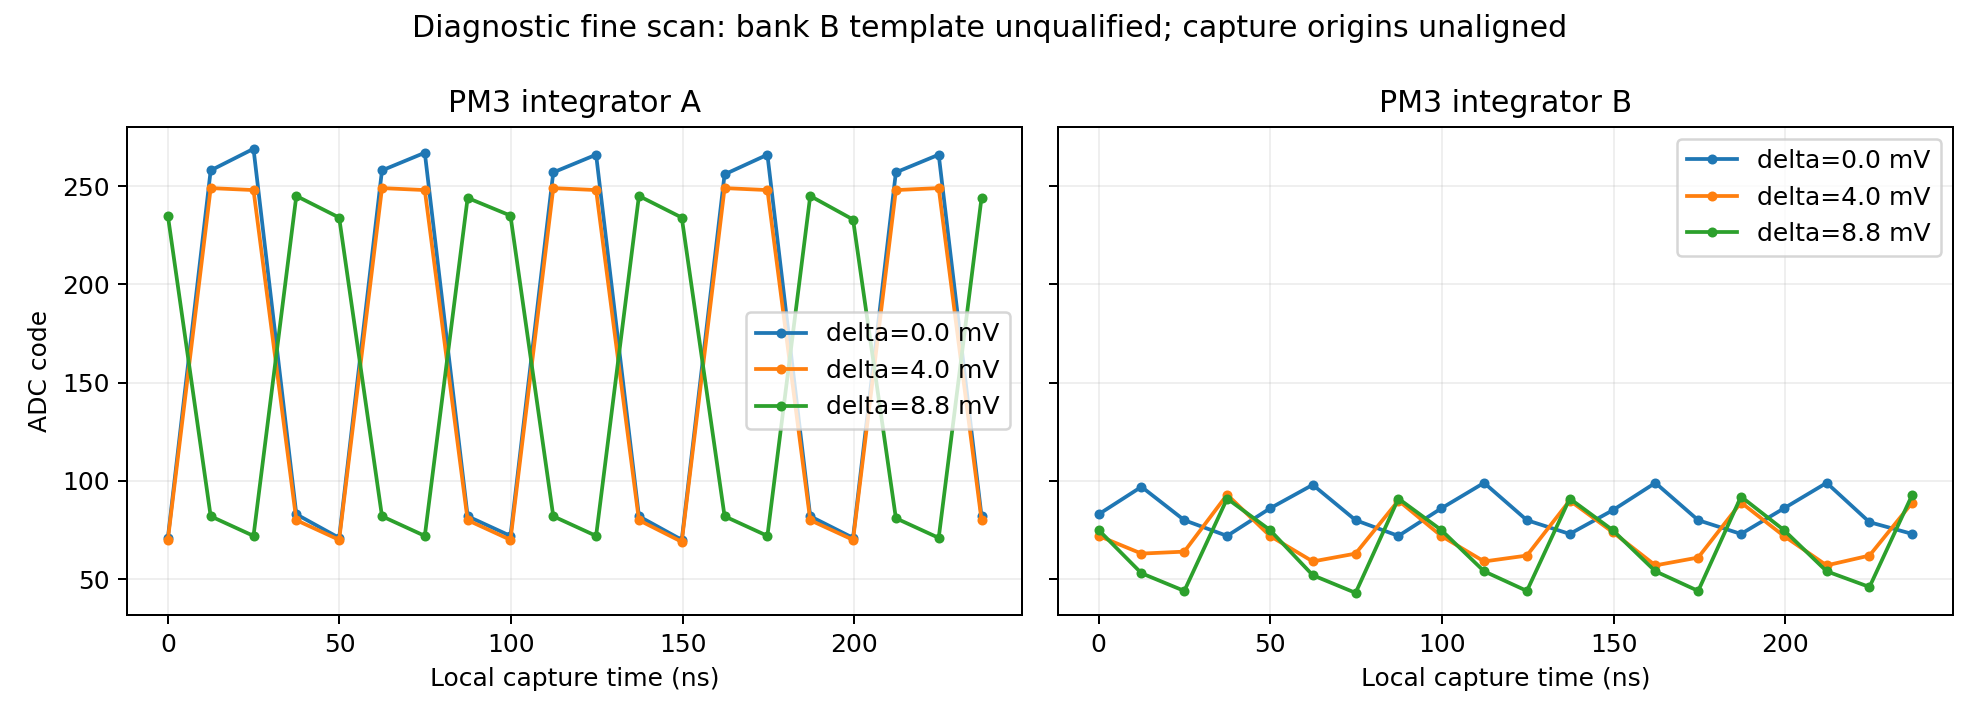
\includegraphics[width=\linewidth]{ch03-integrator3-diagnostic.png}\end{center}
\begin{center}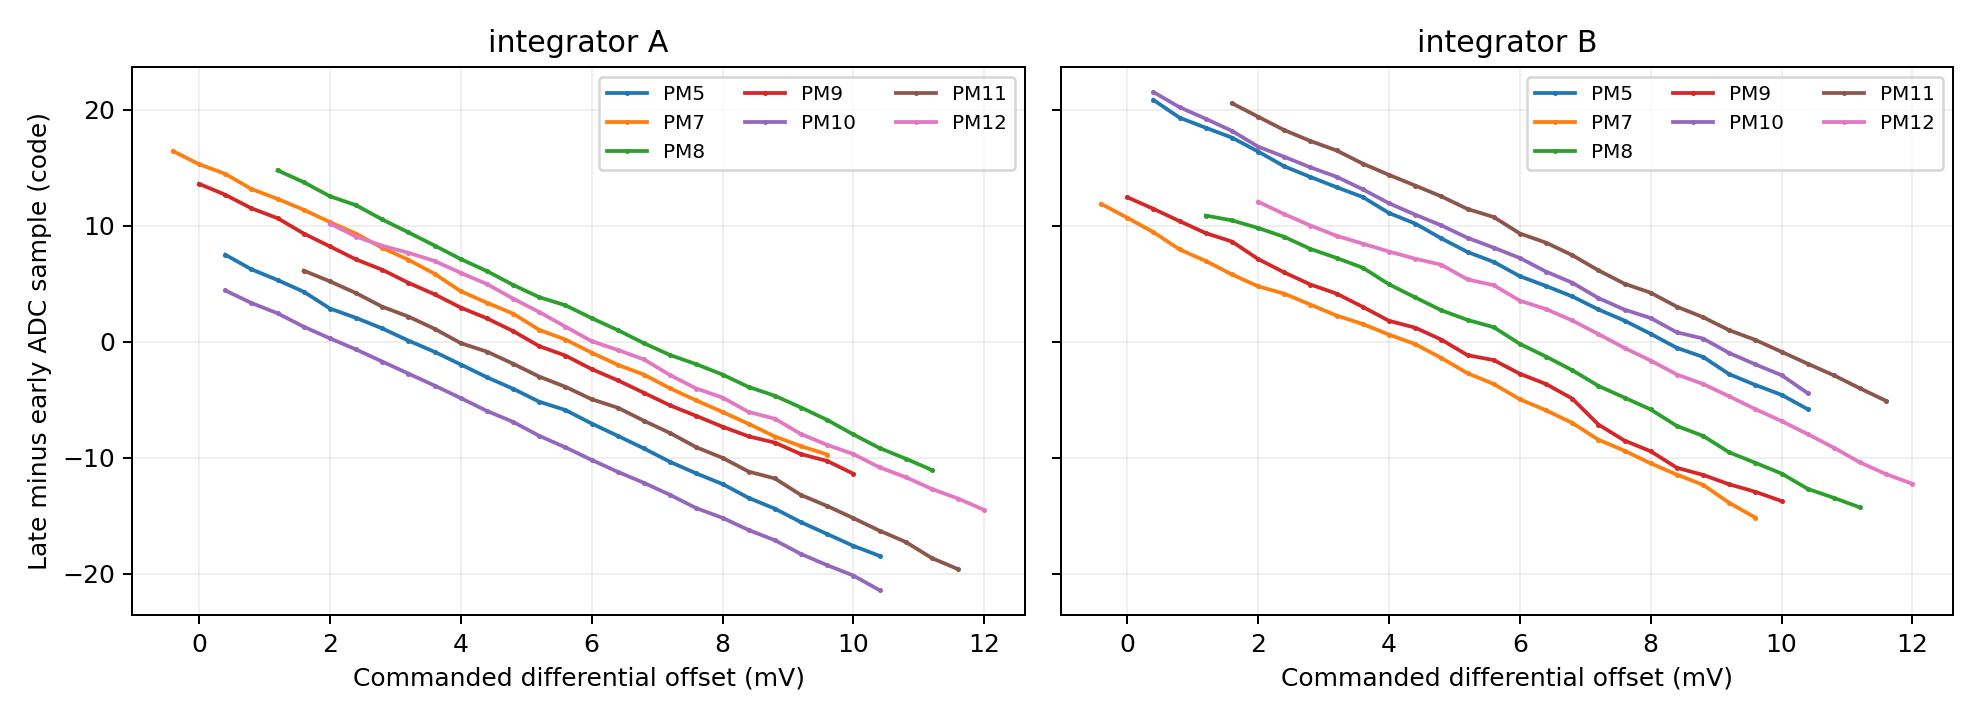
\includegraphics[width=\linewidth]{ch03-integrator-common.png}\end{center}
Only qualified labelled channels are overlaid; incomplete3/4/6 are excluded.
Final amplifiers, direct ADC bypass and monitor muxes inhibited, TCA masks zero;
external DAC0/1 are1/1V and2/3 are1.024/2.048V. Leases released. Analog1--2 awaits USB moves.
\subsection{Zero-input waveforms and FFT, channels3--12}
Independent local capture origins, not synchronized traces. FFT amplitudes are
one-sided RMS code per bin at nominal80.1574MS/s, not PSD or intrinsic aperture jitter.
\begin{center}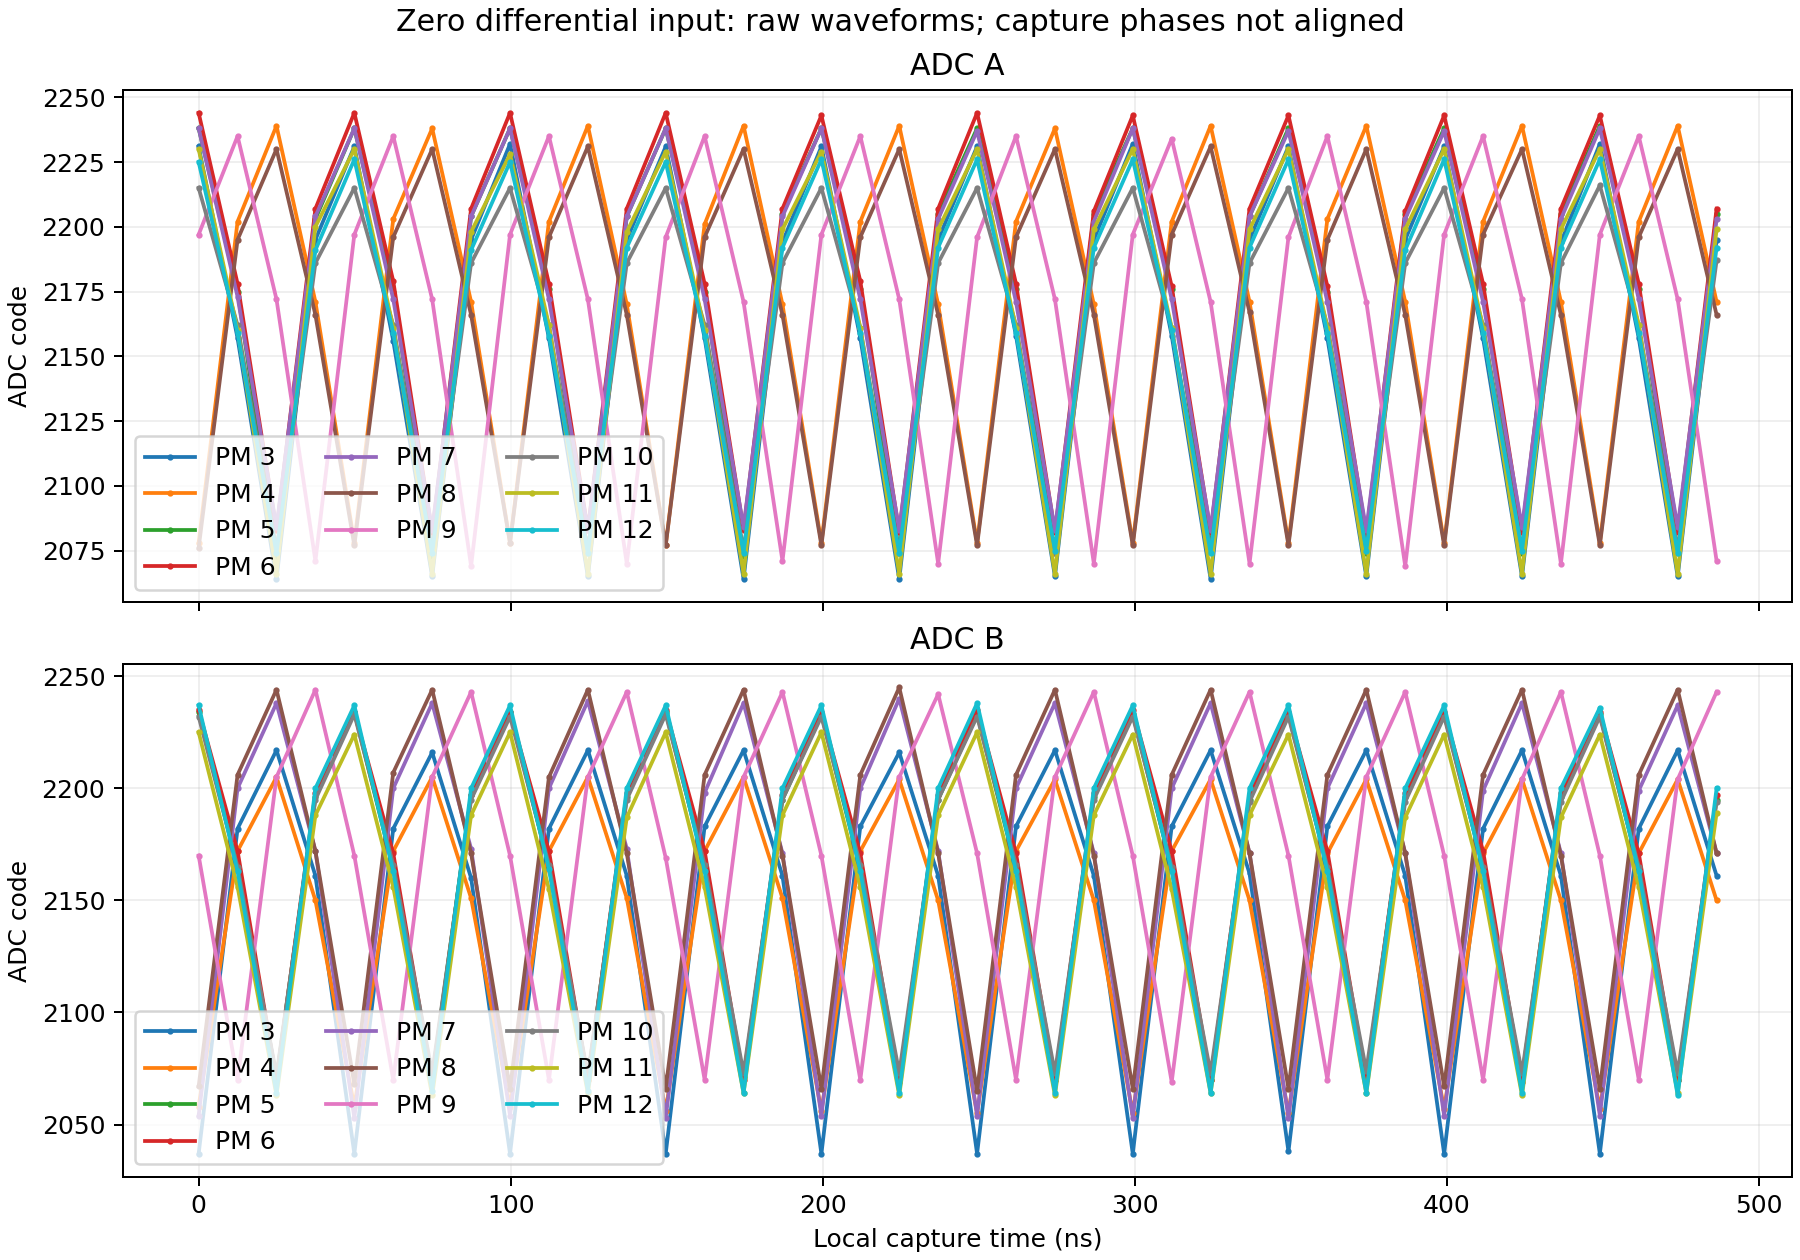
\includegraphics[width=\linewidth]{ch03-adc-zero-time.png}\end{center}
\begin{center}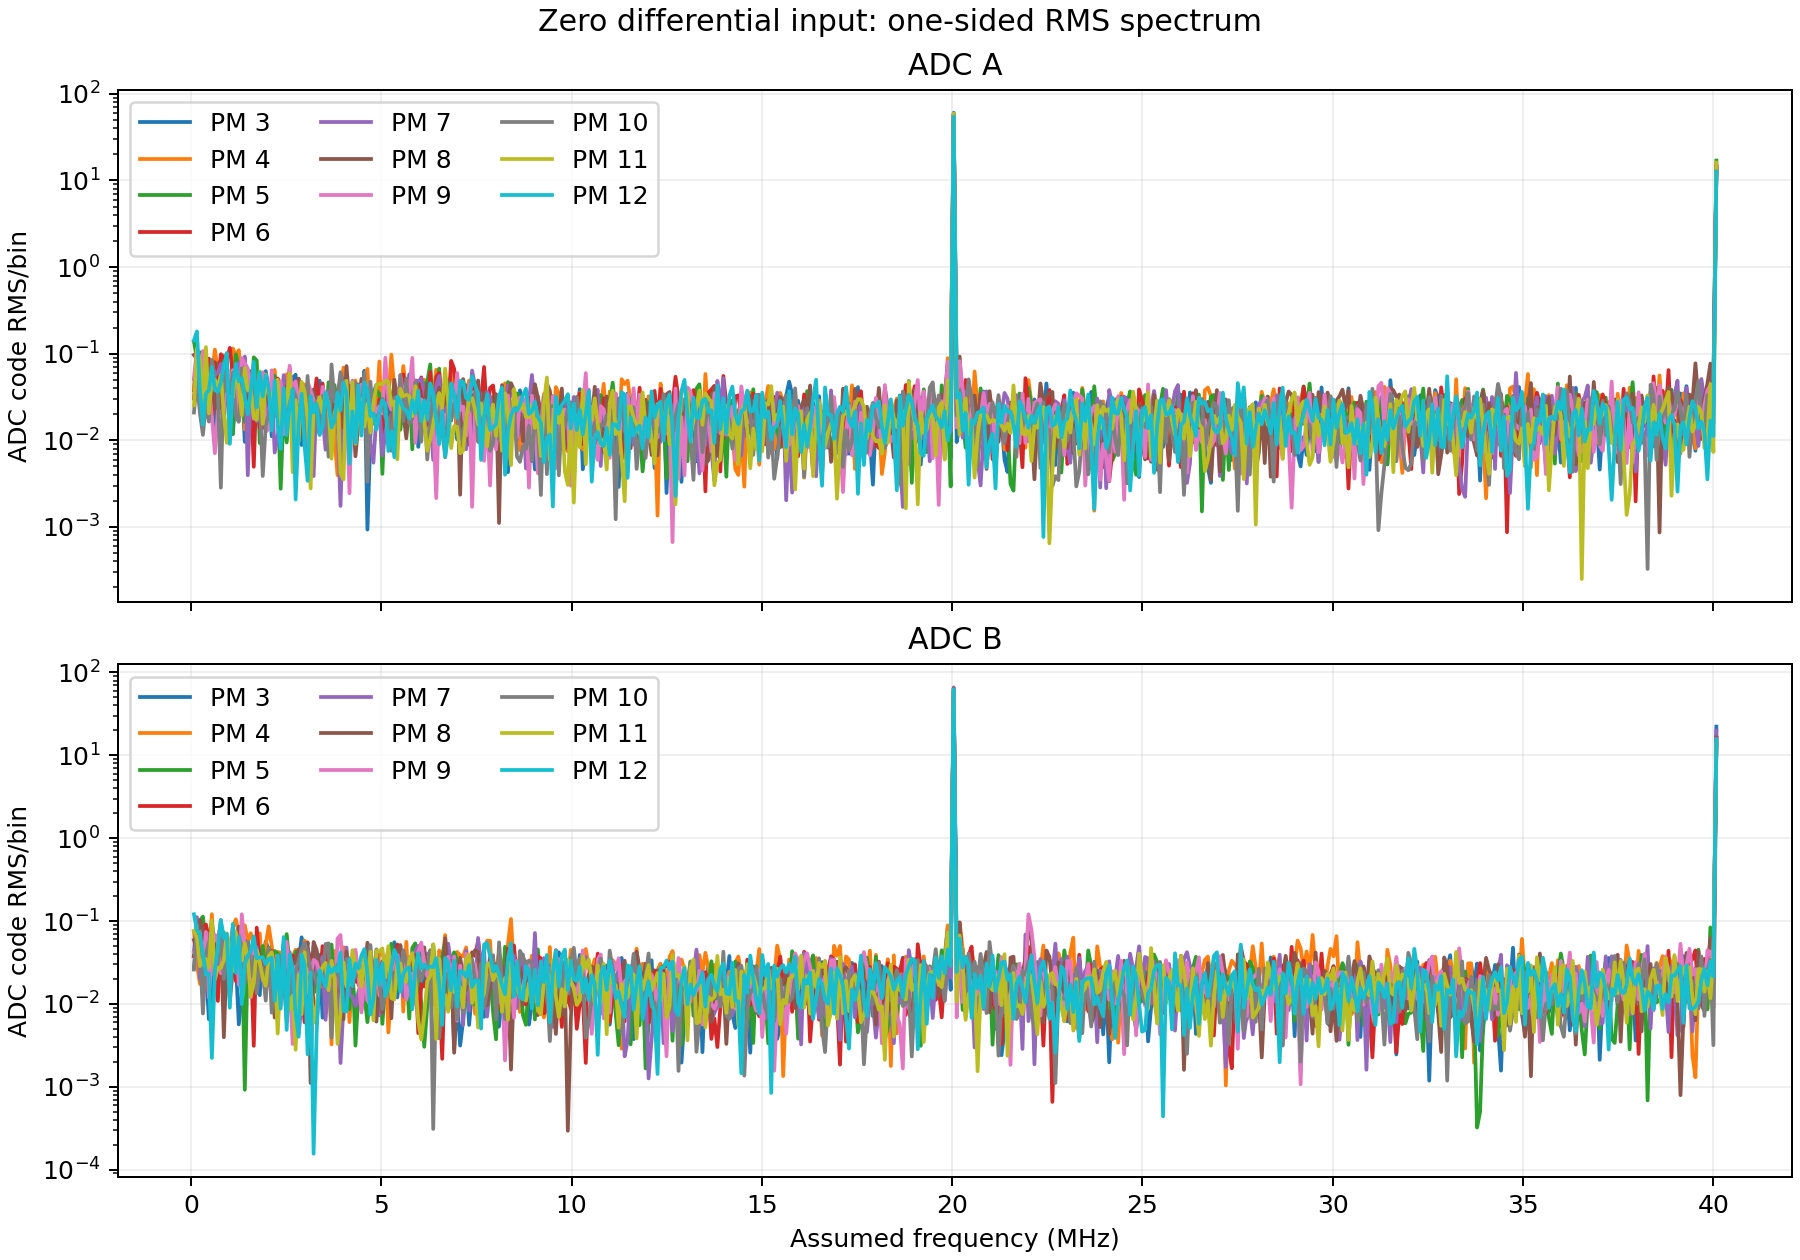
\includegraphics[width=\linewidth]{ch03-adc-zero-fft.png}\end{center}
